\chapter{怎样克服自激振荡}\label{ch5}
\section{自激振荡是怎么回事?}
在正常情况下,如果切断行波管的输入信号,则输出信号设也随之消失。但是,有时也会出现一种反常现象,那就是:当的行波管加上正常工作电压后,虽然没有输入信号,却有高频信雪号输出。这输出信号是从哪里来的呢?原来是管子发生了自激振荡。它的频率可以是单一的,也可能是杂乱的、多频率的。振荡信号的功率可能是微弱的,也可能是很强的,甚至可以与管子的最大输出功率相比拟。一般说来,自激振荡的功率和频率都是不稳定的。


行波管的自激振荡,对管子的正常工作是很有害的。因为这种不稳定的寄生振荡信号对外加的被放大信号是很大的干扰,使行波管不能正常工作。所以,必须设法防止自激振荡的发生,或者把自激振荡的强度限制在极低的电平以下,使它不致影响行波管的正常工作。


下面几节将分别介绍螺旋线型行波管中引起自激振荡的几个常见的、主要的原因以及抑制自激振荡的方法。最后,谈谈自激振荡的判断和测试。


\section{内部反射引起的自激振荡}
产生自激振荡的一个重要原因,是管子的内部反射。我们知道,电磁波在沿传输线传播的途中,如果遇到不均匀的地方(例如接头或介质不均匀处),就会引起反射。行波管的螺旋线是一种特殊的传输线,与螺旋线两端相连接的输能装置便是电磁波在行波管中传播时必然会遇到的不均匀地方。如果输能装置的匹配不良,就会造成严重的反射。即使是匹配较好的输能装置,也不可能做到理想匹配,因此总会造成一定的反射。


内部反射的存在究竟是怎样引起自激振荡的呢?让我们来看看它的产生过程。


如果在行波管的输入端引进一个微弱的高频信号(比如,由于电子注的扰动在输入端就能够激励起频谱很宽的微弱信号),当它沿螺旋线向前传播时,其中某些频率的微弱信号因为与电子注同步因而发生了相互作用,信号得到了放大,但是到达输出端时由于输能装置的不匹配,放大了的信号将有一部分被反射回来,反射回来的信号再沿螺旋线向输入端方向传输,显然,由于它的传播方向与电子注的前进方向相反,不能满足同步条件,因而,它们之间不可能相互作用,反射信号不可能被放大。相反,由于螺旋线的损耗还要衰减掉一部分。衰减后剩下的那部分反射信号在到达输入端时由于输入端的不匹配又会遇到反射。反射信号便将沿着螺旋线与电子注同方向地向前传播。可见,从微弱信号进入输入端到现在正好完成一个循环。可以设想,如果此反射信号比起最初在输入端出现的微弱信号大的话,那么,这个循环过程就能继续下去,输出信号也将逐渐增大,一直达到某一个比较稳定的状态。此时,虽然没有信号输入,但是却有信号输出。这种现象就叫做自激振。

其实,行波管内产生自激振荡的条件和低频下的三极管产生自激振荡的条件是类似的。为了维持振荡就需要满足两个条件,即振幅条件和相位条件。让我们先来看一看振幅条件:假设行波管输入端最初激励起来的微弱信号功率为$ P_i $(如图\ref{ch5-1}所示),行波管的放大倍数为$ G $,那么在输出端将得到放大的信号功率$ P_0 = GP_i $,若输出端的反射系数为$ n_0 $,则反射的那部分信号功率为$ n_0P_0 = n_0GP_i $,如果螺旋线的衰减量为$ L $,那么,反射信号从输出端回到输入端时还剩下$ \frac{1}{L} n_0P_0 = \frac{n_0GP_i}{L}$。在输入端它又遇到了反射,若反射系数为$ n_i $,则其反射功率等于$ n_i\frac{n_0GP_i}{L} $。因此,如能满足下面的条件:

\begin{equation*}
	\frac{n_in_0GP_i}{L > P_i};
\end{equation*}
或\begin{equation} \label{eq:5-1}
	 G > \frac{L}{n_in_0}
\end{equation}
此循环过程才有可能继续下去,这就是产生振荡的振幅条件。

所谓相位条件就是:经过一个循环(即经过输出、输入端两次反射)以后的反射信号与最初在输入端激励的信号应当是同相的。相位条件可以写成下式:

\begin{equation} \label{eq:5-2}
	\beta_0 l +\beta l + \angle n_0 + \angle n_i = 2n\pi
\end{equation}

式中$ \beta_0 l $表示从输出端向输入端传播时的相位移。$ \beta l $则表示从输入端向输出端传播时的相位移。$ \angle n_0 $、$ \angle n_i $分别表示信号输出端及输入端遇到反射时的相位移。$ n $为正整数。


\eqref{eq:5-2}式表明:信号在一个循环中的传播、反射所造成的全部相移之和应当是$ 2\pi $的整数倍。


为了抑止这种由内部反射引起的自激振荡,我们常常采用破坏振幅条件的办法。也就是说,使$ G < \frac{L}{n_in_0} $。现在来设想一个最坏的情况,就是输入端、输出端都是全反射的情况,此时,$ n_0 = n_i = 1 $。因此,如果希望在这种情况下也不产生自激振荡,那么应该有:
\begin{equation} \label{eq:5-3}
	G < L
\end{equation}


我们知道,行波管的增益一般在30\textasciitilde50分贝。因此为了满足上面条件,螺旋线的衰减量$ L $就应该至少大于60\textasciitilde70分贝(为了可靠起见,生产中往往留有十几分贝的余量)。怎样使螺旋线具有这么大的衰减量呢?办法就是在螺旋线当中引入段所谓集中衰减器。它的衰减量很大,例如,可做到60\textasciitilde70分贝以上,但是却集中在很小的一段区域,因此叫做集中衰减器。


下面,我们来介绍一下集中衰减器的制法和它的作用。

图\ref{ch5-2}是行波管集中衰减器的示意图。它的制法是在螺旋线介质夹持杆上距离输入端约1/3全长处,蒸上一层薄薄的吸收物质(例如碳层),其长度通常约为30\textasciitilde40毫米。这样得到的碳膜集中衰减器,其衰减量很容易做到70分贝以上。因此从输出端反射回输入端的高频信号功率便可以基本上全部被吸收掉,这样,便破坏了自激振荡的振幅条件,从而抑止了自激振荡。现在的问题是集中衰减器的出现对于行波管的放大作用会有多大的影响?因为我们是把集中衰减器放在距离输入端约为整个螺旋线长度的$ \frac{1}{3} $地方的,因此,虽然集中衰减器将把从它那里通过的高频信号功率几乎全部吸收掉(集中衰减器既然能够把从输出端反射回来的信号全部吸收掉,那么它也必然能把正向传播的高频信号全部吸收掉,这是一视同仁的),但是它对于在螺旋线中流过的电子注却是无能为力的(实际上,由于集中衰减器并不是集中在一点,因而对电子注将有一定的影响我们将在后面提到它)。经过了$ \frac{1}{3} $螺旋线长度以后,电子注已经得到了一定程度的群聚,即产生了一定程度的密度调制,因此,当电子注穿出集中衰减器以后,便会在其余$ \frac{2}{3} $螺旋线长度内重新激励起新的高频场,并与之发生相互作用、交换能量,使高频场不断放大,最后,我们仍然能够在输出端处得到足够强的高频信号,这就是集中衰减器的好处。试设想,如果把衰减器复盖住从输入端至输出端的整个长度,也就是不把它集中”起来,那么,它不但把从输出端反射回来的信号和正向传播的信号都全部吸收掉,而且使电子注根本无法得到群聚,因此我们便将一无所获,输出信号等于零。


不难想到,集中衰减器的位置将对行波管的增益产生较大的影响。如果集中衰减器距离输入端太近,那么,在较弱的高频场和与之同步的电子注进入集中衰减器时,电子注就会来不及得到足够的群聚,它的密度调制太小,因而在穿出集中衰减器以后便不能有效地在螺旋线上激励起高频场,行波管的增益便大大减小。


另一方面,如果集中衰减器距离输入端太远,那也不好因为这样一来,第\uppercase\expandafter{\romannumeral3}区(见图\ref{ch5-2})的长度就会太短,电子穿出集中衰减器以后没有足够的空间距离与高频场相互作用因而也会使行波管的增益大大降低。


理论计算表明,集中衰减器与输入端的距离(即图\ref{ch5-2}中第\uppercase\expandafter{\romannumeral1}区的长度)应当这样选择,就是使它所包含的波数$ N_1 $满足下列条件:$ CN_1 \ge 0.2 $。在这种条件下,即使在集中衰减器处将螺旋线切断(衰减量为无穷大),增益也不过下降3.52分贝。实际的集中衰减器往往具有一定的轴向长度。我们可以把这段长度看成一段无场的漂移空间,这段漂移空间将对电子注的群聚产生不利的影响(由于空间电荷力的作用),最终也将导致增益的降低。如果我们把集中衰减器的长度和衰减量对增益的影响合起来考虑,那么,总共将使增益降低6分贝左右


有时由于集中衰减器两端的匹配情况不够好,也会在行波管中引起自激振荡。这种新的自激振荡是由于集中衰减器靠近输出端的一侧匹配不良所引起的。由于一方面集中衰减器的匹配不够好,另一方面第\uppercase\expandafter{\romannumeral3}区的增益往往又很高,因此,高频信号就可能在集中衰减器与输出装置之间来回反射而产生振荡这种自激振荡常被我们叫做\uppercase\expandafter{\romannumeral3}区振荡。为了抑止\uppercase\expandafter{\romannumeral3}区振荡,我们采取了一个简便的办法,就是把集中衰减器两端的匹配(特别是靠近输出端的匹配)做得尽可能好(使蒸发在夹持杆上的吸收物质从无到有的渐变段做得尽可能好)。这样,从输出端反射回来的高频信号功率便能几乎全部被集中衰减器所吸收因而有效地抑止了\uppercase\expandafter{\romannumeral3}区振荡。


从上面的介绍我们可以看出,集中衰减器有效地抑止了内部反射所引起的自激振荡。总起来说,对集中衰减器应该有三个要求:(1)衰减量要足够大,通常大于60\textasciitilde70分贝。(2)两端匹配要足够好,通常驻波比(等于$ \frac{1+\textrm{反射系数}}{1-\textrm{反射系数}} $)应优于1.1。(3)集中衰减器的长度要尽可能短以减小对增益的影响。


但是,人们在生产实践中又发现,有些行波管虽然已经装置了性能良好的集中衰减器,却仍然会因内部反射而发生自激振荡!这是为什么呢?经过反复实践才知道,这多半是由于制造行波管时某些零件加工或是部件装配过程中的缺陷所造成的。下面举几个例子说明这种情况:


金属陶瓷结构的中小功率行波管,常采用金属管壳弹性变形的方法来夹持螺旋线慢波系统,这是一种比较简便易行而又性能良好的装配方法。但是,如果装配尺寸不适当而使夹持过紧,或者是金属管壳过份弯曲,则往往使细长、脆弱的夹持杆在一处或几处折断,并进而使夹持杆断裂处的螺旋线受力而局部变形,发生螺距突变,形成电磁波传播路径上的反射点,这些反射点与管子输出端之间构成管内反馈途径,特别是那些处于第\uppercase\expandafter{\romannumeral3}区的反射点,由于和输出端之间不存在集中衰减器,而\uppercase\expandafter{\romannumeral3}区的增益又通常较高,所以很容易引起严重的自激振荡,它的情况与前面介绍的\uppercase\expandafter{\romannumeral3}区振荡很相似。


另一个例子是由于螺旋线绕制精度不高引起自激振荡。绕出的螺距不均匀,螺距突变处就要引起反射。特别是,如果由于绕制设备或其它原因使螺距出现周期性突变,则更易引起自激振荡。因为在这种情况下,某些频率的信号经不同位置上周期性出现的反射点反射后,相位合适时可以在某处互相叠加。尽管每个反射点的反射不太严重,但各点反射信号叠加后就会出现较强的反射信号,它与一个较大的反射点对信号所产生反射的效果相同,所以也会引起可观的自激振荡。


再一个例子是,如果夹持杆对螺旋线的夹持过松,就会因夹持杆上的衰减层与螺旋线接触不紧而使实际衰减量下降,以致不能提供为抑制内部反射振荡所必须的集中衰减量,所以虽然集中衰减器本身的性能是良好的,但仍然会因内部反射而发生自激振荡。


从以上几例可以看出,为了防止行波管中反射引起的自激振荡,不仅要正确设计和制作一个良好的集中衰减器,而且还要通过合理的零件加工和装配精度,设法避免管内以任何形式出现的反射点。

\begin{figure}[phtb]
	\centering
	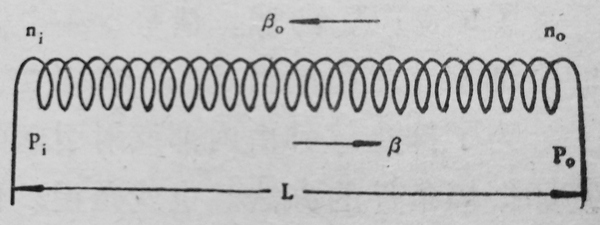
\includegraphics[width=0.55\linewidth]{figure/ch5-1}
	\caption{内部反射引起自激振荡的振幅条件$ G>\frac{L}{n_i n_o} $}
	\label{ch5-1}
\end{figure}

\begin{figure}[phtb]
	\centering
	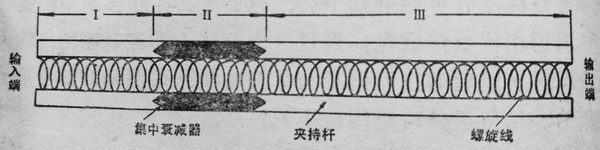
\includegraphics[width=0.65\linewidth]{figure/ch5-2}
	\caption{行波管中的集中衰减器}
	\label{ch5-2}
\end{figure}
\section{外部反馈引起的自激振荡}


管外反馈是引起行波管自激振荡的另一个重要原因。行波管是高增益放大器件。目前,小信号增益达40\textasciitilde50分贝的行波管已比较常见,也就是说,行波管输出与输入电平往往相差几十万倍甚至更大!在这种情况下,输出、输入端之间的外部隔离也成为一个严重问题。一般由于行波管外部结构及输能装置的设计和制造不易做得绝对严密,所以总有部分信号从行波管输出端泄漏出来然后由输入端侵入管内,从而在行波管外部构成一个正反馈回路。如果条件合适就会产生自激振荡。


和内部反馈自激振荡的振幅条件相似,我们得到外部反馈自激振荡的振幅条件为:
\begin{equation} \label{eq:5-4}
	G_{ss} > L_0
\end{equation}

式中$ G_{ss} $为行波管的小信号增益。


$ L_0 $为行波管输入输出之间的外部空间衰减(均以分贝计)。


这种由外部反馈引起的自激振荡,只要找到反馈的途径,然后设法堵住它就可以消除。采取的措施通常是增加外部空间衰减$ L_0 $,使$ L_0 > G_{ss} $来破坏自激振荡的振幅条件。具体的方法是:


(1)增加屏蔽,用导电材料堵住漏隙。


(2)在外部反馈的途径上设置微波吸收材料。


这两种方法都可以有效地增大空间衰减,抑止自激振荡。例如:设计行波管外部结构及输能装置时,应当尽量使得它结构严密,用以增加屏蔽效果。又如,在玻璃行波管管壳外涂敷石墨层,就可以吸收经外部空间向输入端反馈的高频信号。
\section{二次电子引起的自激振荡}
当电子以一定的速度打到金属表面时,从金属表面将有电子反打出来,这些反打出来的电子就叫做二次电子,而最初打到金属表面的电子叫做一次电子。二次电子的多少与金属材料的性质、一次电子的速度等因素有关。二次电子的速度也是各种各样的。


在行波管内,从电子枪发出的电子,在穿过螺旋线并与高频场完成能量交换作用后还剩余很多能量,因而以很高的速度打到收集极上,此时,从收集极表面就会打出很多二次电子它们以不同的速度向四面八方飞去,其中最危险的就是重新飞进螺旋线内并且速度和慢电磁波速度差不多的二次电子(严格地说,还应包括受降压收集极产生的减速电场作用而中途返回螺旋线的一次电子。关于降压收集极,我们将在后面介绍),如图\ref{ch5-3}所示。这些二次电子将在聚束磁场的聚束作用下(聚束磁场对于正向飞行的电子和反向飞行的电子,其聚束作用是相同的)从输出端向输入端飞行,如果此时有从输出端反射回来的高频场沿螺旋线向输入端方向传播,由于两者是同步的,因此它们之间就可以充分地进行能量交换,使得向输入端方向传播的高频场得到放大,我们把它叫做反向放大,其增益称为反向增益。和正向放大一样,集中衰减器对反向增益的影响也(很小。反向放大的存在给自激振荡提供了便利条件。因此,当反向放大倍数足够大的时候,就可能产生可观的自激振荡。通常,在收集极降压(为了降低收集极的功率耗散)的行波管中,如果不采取措施的话,就容易产生由二次电子及返转的一次电子所造成的自激振荡。因为在这种行波管里,从收集极飞出来的二次电子或返转的一次电子在螺旋线电压产生的加速电场作用下,是很容易进入螺旋线内并获得与高频场同步的速度的。降压收集极区域的电位分布见图\ref{ch5-4}所示。


由上面的分析可知,这类自激振荡是由于二次电子进入螺旋线内而引起的(对收集极降压的行波管来说还可能是由返转的一次电子引起的)。因此,为了抑止二次电子所产生的自激振荡,只要想办法阻止二次电子进入螺旋线内就行了。常用的办法有两个:1.改进收集极结构。例如,把收集极做成细口状或内部有一定的锥度的(见图\ref{ch5-5})。这样,二次电子就不容易飞出收集极口,最后它们将仍然落在收集极内表面上。2.改变收集极处的聚束磁场,使得这部分磁场变得不是轴对称的,或者使得这部分磁场的对称轴与原来的对称轴有一个夹角,这样,即使从收集极口能够飞出来的二次电子也因为磁场的偏转作用而无法进入螺旋线内(关于磁场对运动电子的作用将在第\ref{ch7}章中讲述)。实践证明上面两个方法对于抑止二次电子产生的自激振荡是行之有效的。采用这两个办法以后,即使对于收集极降压的行波管,我们也能有效地抑止二次电子及返转的一次电子引起的自激振荡。


附带指出,行波管内还可能由于返波的存在而产生振荡即返波振荡。关于返波振荡,因为在中小功率行波管中基本上不会碰到,而且很容易通过螺旋线的正确设计来避免(即保证$ ka < 0.3 $),因此不多介绍。


\begin{figure}[phtb]
	\centering
	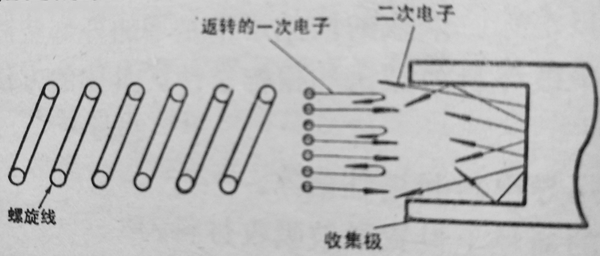
\includegraphics[width=0.65\linewidth]{figure/ch5-3}
	\caption{二次电子和反转的一次电子进入螺旋线}
	\label{ch5-3}
\end{figure}

\begin{figure}[phtb]
	\centering
	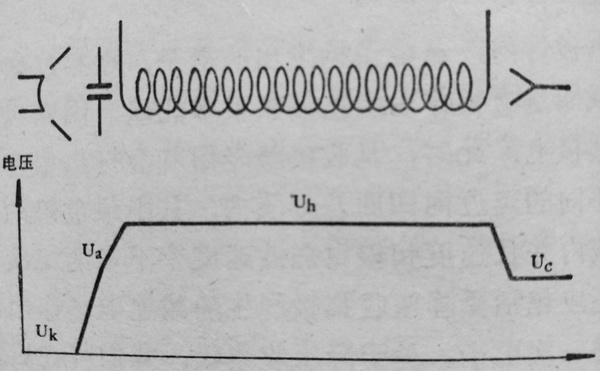
\includegraphics[width=0.62\linewidth]{figure/ch5-4}
	\caption{收集极降压行波管的电位分布}
	\label{ch5-4}
\end{figure}

\begin{figure}[phtb]
	\centering
	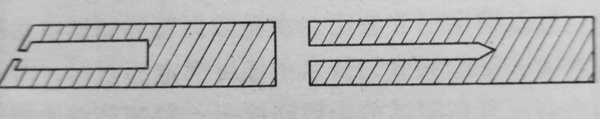
\includegraphics[width=0.65\linewidth]{figure/ch5-5}
	\caption{改进收集极结构}
	\label{ch5-5}
\end{figure}
\section{怎样判断自激振荡?}
在行波管出现自激振荡以后,首先需要判断一下它是属于哪一类的,以便对症下药,采取相应的措施来抑止它。图\ref{ch5-6}是自激振荡的测试方框图。


输出端及输入端都接有定向耦合器和功率计,它们是用来分别观察出现在两端的自激振荡功率大小的。


我们知道,在自激振荡的振幅条件中,输入输出端的反射情况占有重要的地位。为了保证在最坏的运用情况下仍不致引起自激振荡,我们常常在行波管的技术条件中规定一个最坏运用情况下的输入输出端驻波比。在自激振荡的测试中就需要把输入输出端的驻波比调节到技术条件所规定的指标,因此需接以驻波引入器,并在测试前先把驻波引入器的驻波比调节到规定的数值。最严格的要求是在两端全反射的情况下也不出现振荡,这时可在输入输出端都接以短路器来检查有无振荡,人们常说的行波管的短路稳定性就是指输入输出端都接以短路器时管子是否能够稳定地工作。


自激振荡的测试并不复杂。首先把各仪表和元件按图\ref{ch5-6}接好,开启功率计让它预热,然后便可接通被测行波管电调到所需要的收集极工作电流,开始测试。测试时需一边使螺旋线电压在规定范围内扫动(即使其达到同步,以满足振荡的振幅条件),一边调节输入输出端驻波引入器(或短路器)的相位(应使相位变化不小于360\textdegree,以提供振荡的各种相位条件),如功率计有指示,就说明被测管有自激振荡产生如何判断自激振荡产生的原因呢?如果自激振荡的功率相当大(甚至可以和正常的输出功率相比拟),那么,很可能是由内部反射或外部反馈引起的。内部反射有两种情况,一种是集中衰减器衰减量不够而在整个螺旋线长度内产生的振荡。另一种是由于集中衰减器靠近输出端的一端的匹配不够好,因而在第区内来回反射产生了振荡。这两种情况的判断方法是首先改变输入输出端驻波引入器的相位,观察对自激振荡功率的影响。如果是前一种情况,则输入输出驻波引入器的相位对自激振荡功率都有影响,输出端的驻波引入器影响较大。其次,最好测一下集中衰减器的冷衰减量,若衰减量不够大(通常应比该管增益大20分贝以上)且输入输出端驻波引入器都有影响,那就可以肯定是由于管内整个螺旋线长度的内部反射(即输入端和输出端之间的内部反射)引起的自激振荡。如果输入端驻波引入器的相位变化对于振荡功率毫无影响,而输出端驻波引入器的相位对于振荡功率的影响很大,则可能是内部反射引起的\uppercase\expandafter{\romannumeral3}区振荡。上面两种内部反射引起的自激振荡通常是无法消除的,只能在制管过程中加以避免。


自激振荡还常常可能由外部反馈引起。这主要是因为输出端的输能装置不够严密,因而有部分高频功率泄漏到管外,并通过一些途径(如管壳和包装体之间的缝隙)反馈到输入端这样构成了一个外部反馈的道路,因而产生了自激振荡。此时,输入输出驻波引入器的相位变化对自激振荡都有影响,但集中衰减器的衰减量往往是够的。外部反馈产生的自激振荡原则上是可以消除的,只要我们找到输出端功率泄漏的确切途径并加以堵截(如用吸收物质)即可。常用的吸收物质是用石墨填充的泡沫塑料。


二次电子所引起的自激振荡通常不很大。为了判断是否这种振荡,我们可以把收集极电压短时间提高一下,观察功率计的指示是否变小或消失,有时提高收集极电压以后往往可以把二次电子或返转的一次电子引起的自激振荡消除掉,这是因为收集极电压提高后将使螺旋线和收集极之间的电场变得不利于二次电子进入螺旋线方向的运动,因而消除了自激振荡。还有一种判断二次电子引起的自激振荡用的方法,就是用铁磁性物质在收集极附近扰动,若自激功率发生变化就说明二次电子或返转的一次电子参予了自激振荡。当然,不管是提高收集极电压也好,铁磁性物质扰动也好,只能起判别自激振荡是否二次电子或返转的一次电子产生的作用。要消除二次电子引起的自激振荡还需在管子的结构上下功夫,如改进收集极、改进收集极附近的磁聚束系统等。


有时,行波管的自激振荡是由好几种原因产生的,现象要复杂一点,因此,判断起来就不那么简单了。但是,我们总是可以根据各种振荡的性质、特点找出占主要地位的原因然后加以解决的。






\begin{figure}[phtb]
	\centering
	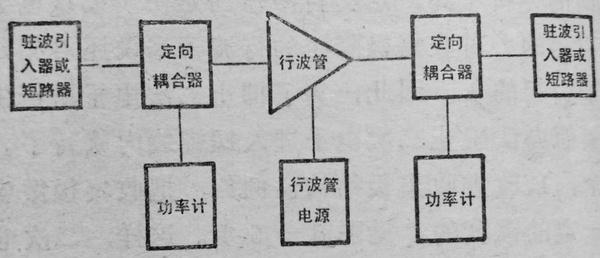
\includegraphics[width=0.65\linewidth]{figure/ch5-6}
	\caption{行波管自激振荡测试方框图}
	\label{ch5-6}
\end{figure}